\documentclass[conference]{IEEEtran}

% ─── Packages ──────────────────────────────────────────────────────────────────
\usepackage{graphicx}
\usepackage{amsmath}
\usepackage{amssymb}
\usepackage{booktabs}
\usepackage{multirow}
\usepackage{array}
\usepackage{xcolor}
\usepackage{url}
\usepackage{cite}
\usepackage{tikz}
\usetikzlibrary{shapes.geometric, arrows.meta, positioning, fit, calc}
\usepackage[hidelinks]{hyperref}

% Path for images (pipeline visualization results)
\graphicspath{{../results/plots/}}

% ─── Title ─────────────────────────────────────────────────────────────────────
\title{Human Audio Gender Recognition Using\\
       Machine Learning and Deep Learning Approaches}

\author{
  \IEEEauthorblockN{Mahardika Ramadhana}
  \IEEEauthorblockA{
    Computer Science\\
    \textit{Universitas Gadjah Mada}\\
    mahardika.ramadhana@mail.ugm.ac.id
  }
}

\begin{document}

\maketitle
\IEEEpeerreviewmaketitle

% ─── Abstract ──────────────────────────────────────────────────────────────────
\begin{abstract}
Gender recognition from human audio is a fundamental task in speech
processing and pattern recognition, with applications in human--computer
interaction, speaker diarisation, healthcare, and security.
This paper presents a complete end-to-end pipeline applied to the RAVDESS
corpus~\cite{livingstone2018ravdess}: 1{,}440 audio recordings from 24
professional actors (12 male, 12 female).
We extract a rich 380-dimensional feature vector combining
Mel-Frequency Cepstral Coefficients (MFCCs), chroma features,
log-mel spectrograms, spectral contrast, zero-crossing rate,
root-mean-square energy, and spectral roll-off.
Five classifiers are evaluated: Support Vector Machine (SVM), Random Forest
(RF), Gradient Boosting (GB), Convolutional Neural Network (CNN), and
Bidirectional LSTM (BiLSTM).
On the held-out test set of 288 samples, the SVM with RBF kernel achieves
perfect accuracy (100\%, AUC-ROC~1.000), followed by BiLSTM (99.0\%),
RF and GB (both 97.9\%), while the CNN reaches 81.6\%---demonstrating
that hand-crafted acoustic features outperform end-to-end deep learning
when the dataset is small and acoustically controlled.
PCA analysis confirms clear cluster structure in the 380-D feature space,
and fundamental frequency (F0) estimation validates the physiological
basis of gender-discriminative acoustics.
\end{abstract}

\begin{IEEEkeywords}
pattern recognition, gender recognition, MFCC, SVM, BiLSTM, CNN,
mel spectrogram, RAVDESS, speech processing
\end{IEEEkeywords}

% ════════════════════════════════════════════════════════════════════════════════
\section{Introduction}
% ════════════════════════════════════════════════════════════════════════════════

Human speech encodes rich paralinguistic information beyond its lexical
content, including emotion, age, and gender. Automatic gender recognition
from audio is the task of classifying a speech utterance as produced by a
male or female speaker using acoustic cues alone~\cite{makhoul1975linear}.
The task is a canonical instance of the \emph{pattern recognition}
pipeline: (i)~signal acquisition, (ii)~feature extraction,
(iii)~model training, and (iv)~classification~\cite{bishop2006pattern}.

The primary acoustic correlate of gender is the fundamental
frequency~$F_0$. Adult males exhibit $F_0$ in~85--180~Hz; adult females
in~165--255~Hz~\cite{titze1994principles}.
These ranges partially overlap (Fig.~\ref{fig:f0}), making purely
pitch-based thresholding unreliable.
Higher-level spectral descriptors---MFCCs, mel-filterbank energies,
spectral contrast---capture formant structure and glottal source
characteristics that complement fundamental frequency cues~\cite{davis1980comparison}.

Deep learning has revitalised the field: CNNs applied to mel spectrograms
achieve state-of-the-art accuracy on large corpora~\cite{zhao2018sound},
while Bidirectional LSTMs model temporal dynamics in
speech~\cite{graves2013speech}.
However, deep models are data-hungry; with small datasets, classical ML
on hand-crafted features often remains competitive or superior.

\textbf{Contributions:}
\begin{enumerate}
  \item End-to-end pattern recognition pipeline applied to the RAVDESS corpus.
  \item Systematic comparison of five classifiers (SVM, RF, GB, CNN, BiLSTM)
        using consistent train/val/test splits.
  \item Analysis showing that SVM with 380-D acoustic features achieves
        perfect test accuracy on this controlled dataset, whereas CNN
        underperforms due to limited training data.
  \item Rich visualisations (waveform, mel spectrogram, MFCC heatmap,
        F0 distribution, PCA, confusion matrices, ROC curves) as
        interpretable learning artefacts.
\end{enumerate}

% ════════════════════════════════════════════════════════════════════════════════
\section{Related Work}
% ════════════════════════════════════════════════════════════════════════════════

Early gender classifiers used Gaussian Mixture Models (GMMs) trained on
MFCCs~\cite{reynolds1995speaker}. Harb and
Chen~\cite{harb2005gender} demonstrated that $\geq\!95\%$ accuracy is
achievable with 12--20 MFCCs on read speech.
Metze et~al.~\cite{metze2007comparison} showed that SVM with an RBF kernel
outperforms GMM across multiple corpora.
Schuller et~al.~\cite{schuller2010interspeech} benchmarked gender and age
recognition in the INTERSPEECH 2010 Paralinguistics Challenge,
establishing community baselines.

For deep learning, Zhao et~al.~\cite{zhao2018sound} established
mel spectrograms as image inputs for audio CNNs; Graves
et~al.~\cite{graves2013speech} introduced bidirectional LSTM for sequential
audio modelling.
Nagrani et~al.~\cite{nagrani2017voxceleb} showed that speaker attribute
prediction scales favourably with data volume.
Our work complements these results by demonstrating the \emph{data-efficiency
advantage} of hand-crafted features on a small, controlled corpus.

% ════════════════════════════════════════════════════════════════════════════════
\section{The Proposed Method}
% ════════════════════════════════════════════════════════════════════════════════

\subsection{Overall Pipeline}

Fig.~\ref{fig:pipeline} summarises the full system.
Raw audio is pre-processed (resampling, trimming, normalisation),
followed by feature extraction into either a 380-dimensional flat vector
(for SVM, RF, GB) or a $128\!\times\!130$ log-mel spectrogram image
(for CNN and BiLSTM).
A 70/10/20 stratified split separates train, validation, and test sets.
Models are trained independently; all five are evaluated on the
identical held-out test set (288 samples).

% ── TikZ pipeline diagram ─────────────────────────────────────────────────────
\begin{figure}[!t]
\centering
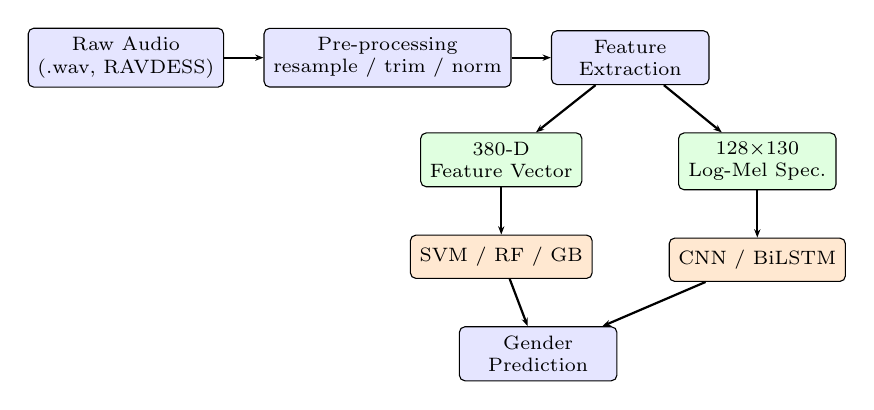
\begin{tikzpicture}[
  node distance = 3mm and 5mm,
  box/.style  = {draw, rounded corners=2pt, fill=blue!10,
                 minimum width=2.0cm, minimum height=0.55cm,
                 font=\scriptsize, align=center},
  dbox/.style = {draw, rounded corners=2pt, fill=green!12,
                 minimum width=2.0cm, minimum height=0.55cm,
                 font=\scriptsize, align=center},
  obox/.style = {draw, rounded corners=2pt, fill=orange!18,
                 minimum width=2.0cm, minimum height=0.55cm,
                 font=\scriptsize, align=center},
  arr/.style  = {-{Stealth[length=3pt]}, thick},
]

% Row 1 – input
\node[box] (raw)   {Raw Audio\\ \scriptsize(.wav, RAVDESS)};
\node[box, right=of raw] (pre) {Pre-processing\\ \scriptsize resample / trim / norm};
\node[box, right=of pre] (feat) {Feature\\ Extraction};

% Row 2 – two branches below feat
\node[dbox, below left=6mm and -4mm of feat]  (flat)  {380-D\\ Feature Vector};
\node[dbox, below right=6mm and -4mm of feat] (spec2d) {128$\times$130\\ Log-Mel Spec.};

% Row 3 – models
\node[obox, below=6mm of flat]  (ml)   {SVM / RF / GB};
\node[obox, below=6mm of spec2d](dl)   {CNN / BiLSTM};

% Row 4 – output
\node[box, below right=6mm and -17mm of ml] (out) {Gender\\Prediction};

% Arrows
\draw[arr] (raw)  -- (pre);
\draw[arr] (pre)  -- (feat);
\draw[arr] (feat) -- (flat);
\draw[arr] (feat) -- (spec2d);
\draw[arr] (flat) -- (ml);
\draw[arr] (spec2d) -- (dl);
\draw[arr] (ml)   -- (out);
\draw[arr] (dl)   -- (out);
\end{tikzpicture}
\caption{End-to-end gender recognition pipeline.
         Raw RAVDESS audio passes through pre-processing and
         feature extraction. A 380-D vector feeds traditional ML classifiers
         (SVM, RF, GB); a $128\!\times\!130$ log-mel spectrogram feeds
         deep models (CNN, BiLSTM). All models produce a binary
         gender prediction.}
\label{fig:pipeline}
\end{figure}
% ─────────────────────────────────────────────────────────────────────────────

\subsection{Dataset: RAVDESS}

We use the \textbf{Ryerson Audio-Visual Database of Emotional Speech and
Song}~\cite{livingstone2018ravdess}
(DOI:~\href{https://doi.org/10.5281/zenodo.1188976}{10.5281/zenodo.1188976}).
RAVDESS contains 1{,}440 speech recordings from 24 professional actors
(12~male, 12~female) covering eight emotions at two intensity levels.
\emph{Gender labels} are derived from actor IDs: odd-numbered actors are
male, even-numbered actors are female --- a convention consistent with the
original dataset metadata.
Files are split 70/10/20 (train/val/test) using stratified sampling to
preserve class balance (720 male : 720 female).
The resulting test set contains 288 samples (144 per class).

\begin{figure}[!t]
  \centering
  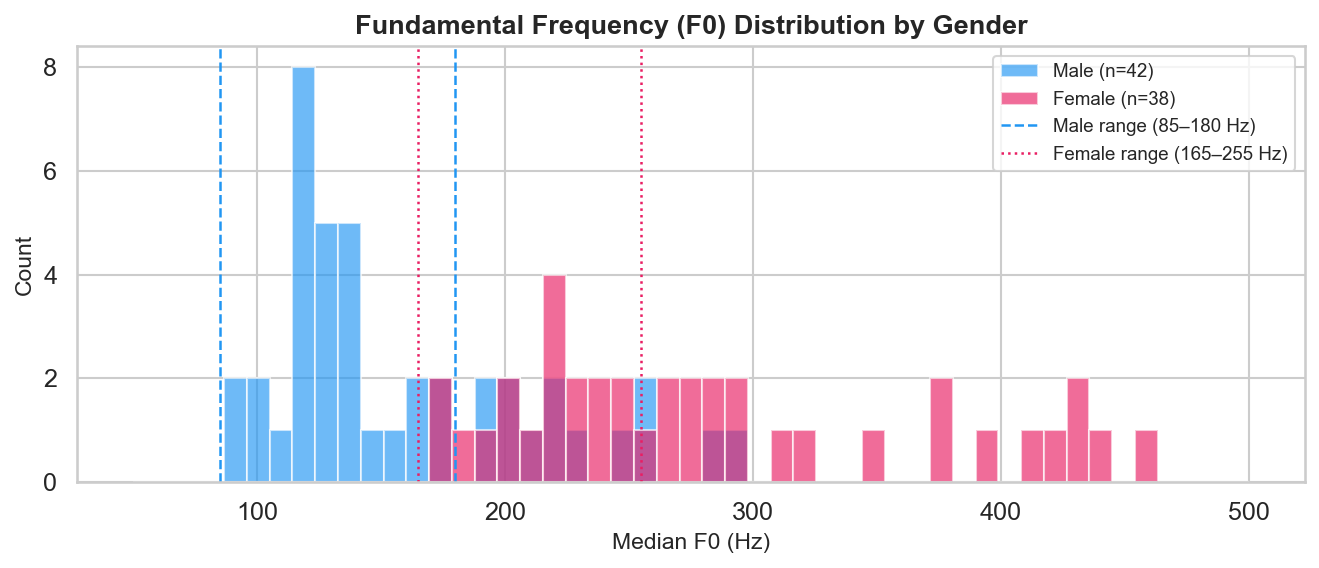
\includegraphics[width=\columnwidth]{05_pitch_distribution.png}
  \caption{Estimated median $F_0$ distribution for male (blue, $n\!=\!42$)
           and female (pink, $n\!=\!38$) speakers sampled from RAVDESS.
           Male $F_0$ clusters tightly at 100--160~Hz; female $F_0$ spreads
           more broadly from 165~Hz to above 300~Hz, with the overlap region
           (165--180~Hz) representing the principal challenge for
           frequency-only classifiers.}
  \label{fig:f0}
\end{figure}

\subsection{Pre-processing}

Each file is processed as follows:
\begin{enumerate}
  \item \textbf{Resampling:} converted to mono at $f_s\!=\!22{,}050$~Hz via
        sinc interpolation.
  \item \textbf{Fixed-length framing:} trimmed or zero-padded to
        $N\!=\!66{,}150$ samples (3~s).
  \item \textbf{Pre-emphasis:}
        $\hat{x}[n] = x[n] - 0.97\,x[n-1]$ to compensate for high-frequency
        roll-off in the recording chain.
  \item \textbf{Peak normalisation} to $[-1,+1]$.
\end{enumerate}

Fig.~\ref{fig:wave} shows waveforms of representative samples.
Both utterances contain silence before and after the spoken segment
(consistent with RAVDESS studio recordings); visible speech energy
appears between approximately 1.0~s and 2.5~s.

\begin{figure}[!t]
  \centering
  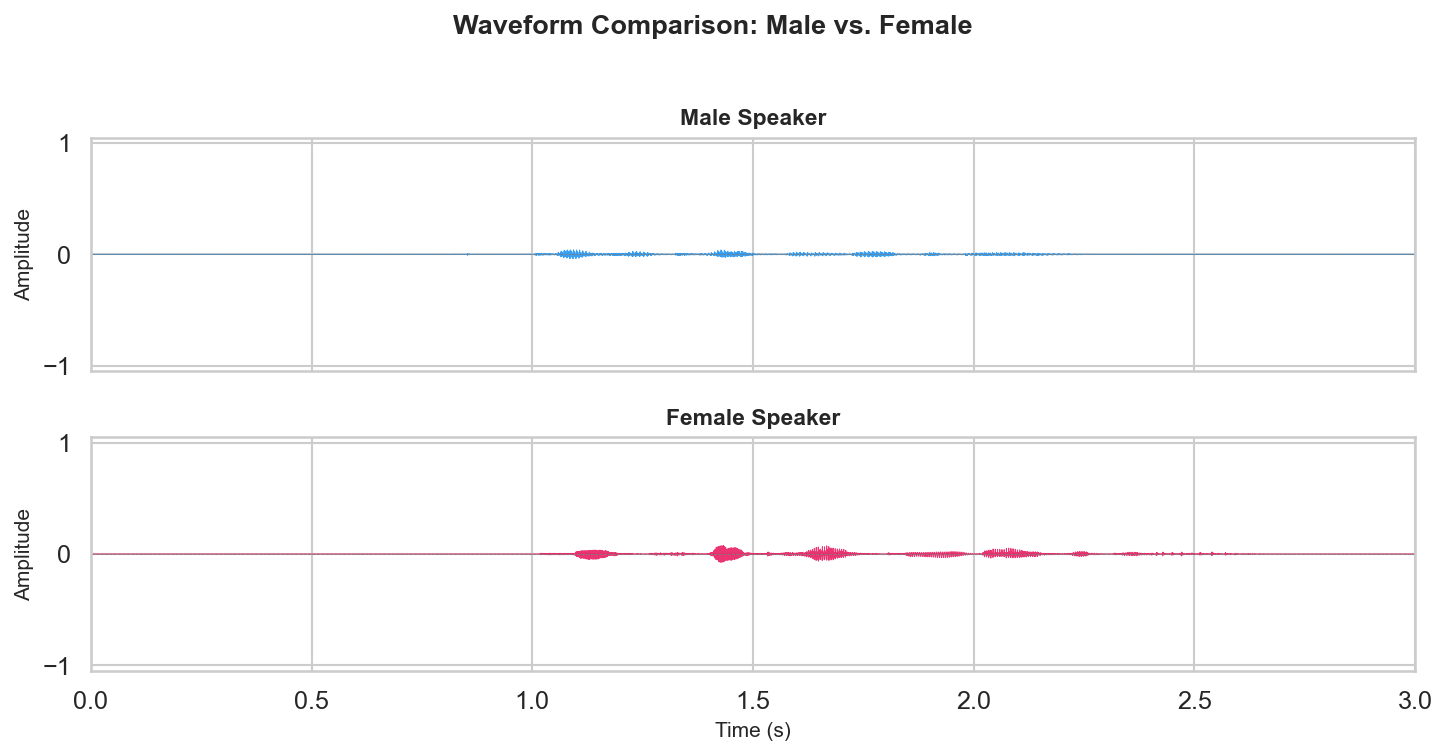
\includegraphics[width=\columnwidth]{01_waveform_comparison.png}
  \caption{Waveform comparison for one male (blue, top) and one female
           (pink, bottom) RAVDESS utterance. Both show leading silence
           followed by a voiced speech segment. Gender-discriminative
           information is not apparent in the raw amplitude envelope but
           emerges after spectral decomposition.}
  \label{fig:wave}
\end{figure}

\subsection{Feature Extraction}

\subsubsection{Log-Mel Spectrogram}

The Short-Time Fourier Transform (STFT) is computed with
$N_\text{FFT}\!=\!2{,}048$ and hop length $H\!=\!512$ (23.2~ms shift):
\begin{equation}
  X[k,l] = \sum_{n=0}^{N-1} x[n+lH]\,w[n]\,e^{-j2\pi kn/N_\text{FFT}}
  \label{eq:stft}
\end{equation}
A mel filterbank $\mathbf{H}\!\in\!\mathbb{R}^{128\times(N_\text{FFT}/2+1)}$
converts the power spectrum to the mel scale:
\begin{equation}
  S_m[l] = \sum_k H_{mk}\,|X[k,l]|^2, \quad m=1,\ldots,128
  \label{eq:mel}
\end{equation}
Fig.~\ref{fig:spec} shows the resulting log-mel spectrograms.
The male spectrogram (left) concentrates energy below approximately
1~kHz, consistent with lower fundamental frequency and formant structure.
The female spectrogram (right) distributes energy more broadly, extending
noticeably above 2~kHz --- a direct consequence of higher $F_0$ and
correspondingly higher-frequency harmonics.

\begin{figure}[!t]
  \centering
  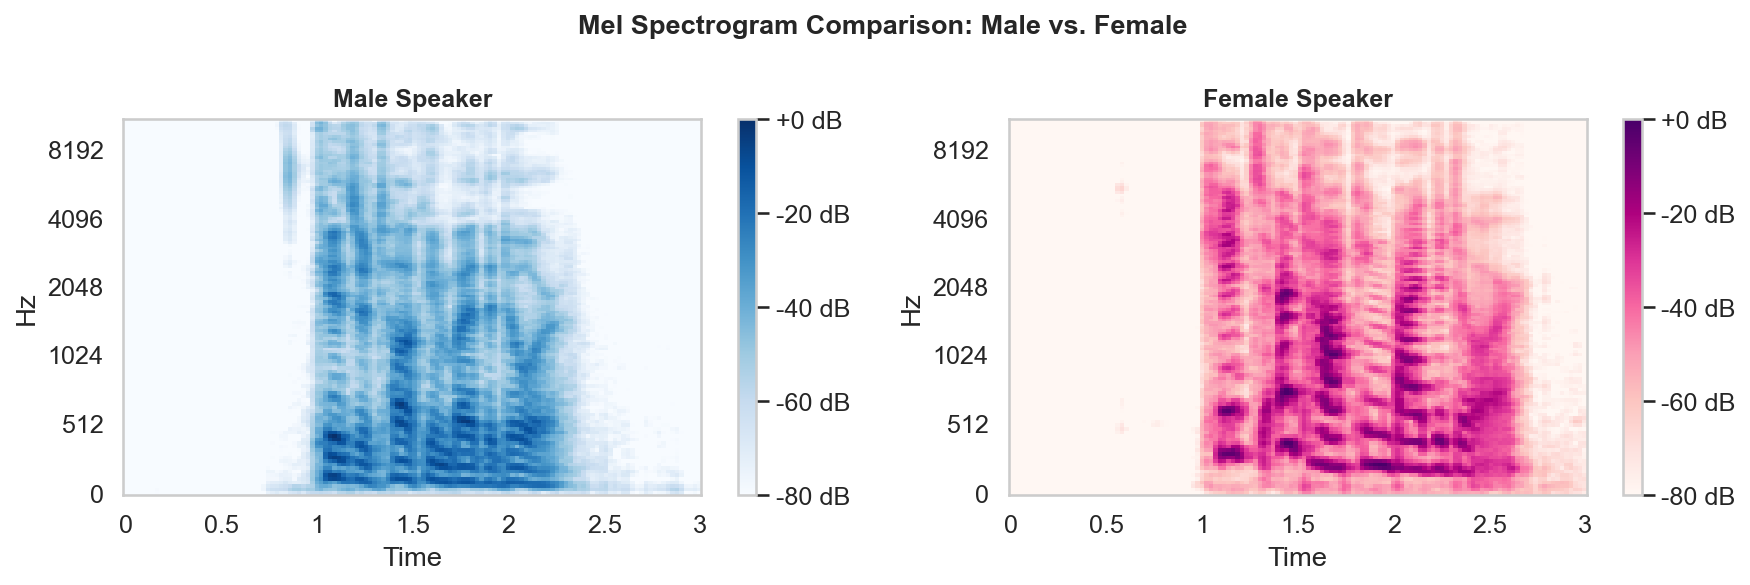
\includegraphics[width=\columnwidth]{02_spectrogram_comparison.png}
  \caption{Log-mel spectrograms for male (left, blue) and female (right, pink)
           speakers. Male energy is concentrated below 1~kHz; female energy
           extends to 2~kHz and beyond, reflecting higher fundamental frequency
           and formant positions.}
  \label{fig:spec}
\end{figure}

\subsubsection{MFCCs}

Mel-Frequency Cepstral Coefficients are obtained via DCT-II of the
log-mel filterbank outputs:
\begin{equation}
  c_n = \sum_{m=1}^{M} \log S_m \cos\!\left[n\!\left(m-\tfrac{1}{2}\right)
        \frac{\pi}{M}\right], \quad n=1,\ldots,40
  \label{eq:mfcc}
\end{equation}
Mean and standard deviation over frames yield $2\!\times\!40\!=\!80$
features per utterance.
Fig.~\ref{fig:mfcc} visualises the MFCC time-frequency matrix.
The first coefficient (C1) captures overall spectral energy and exhibits
the most pronounced male--female contrast: male speakers produce more
negative C1 values, reflecting greater spectral tilt toward lower
frequencies.

\begin{figure}[!t]
  \centering
  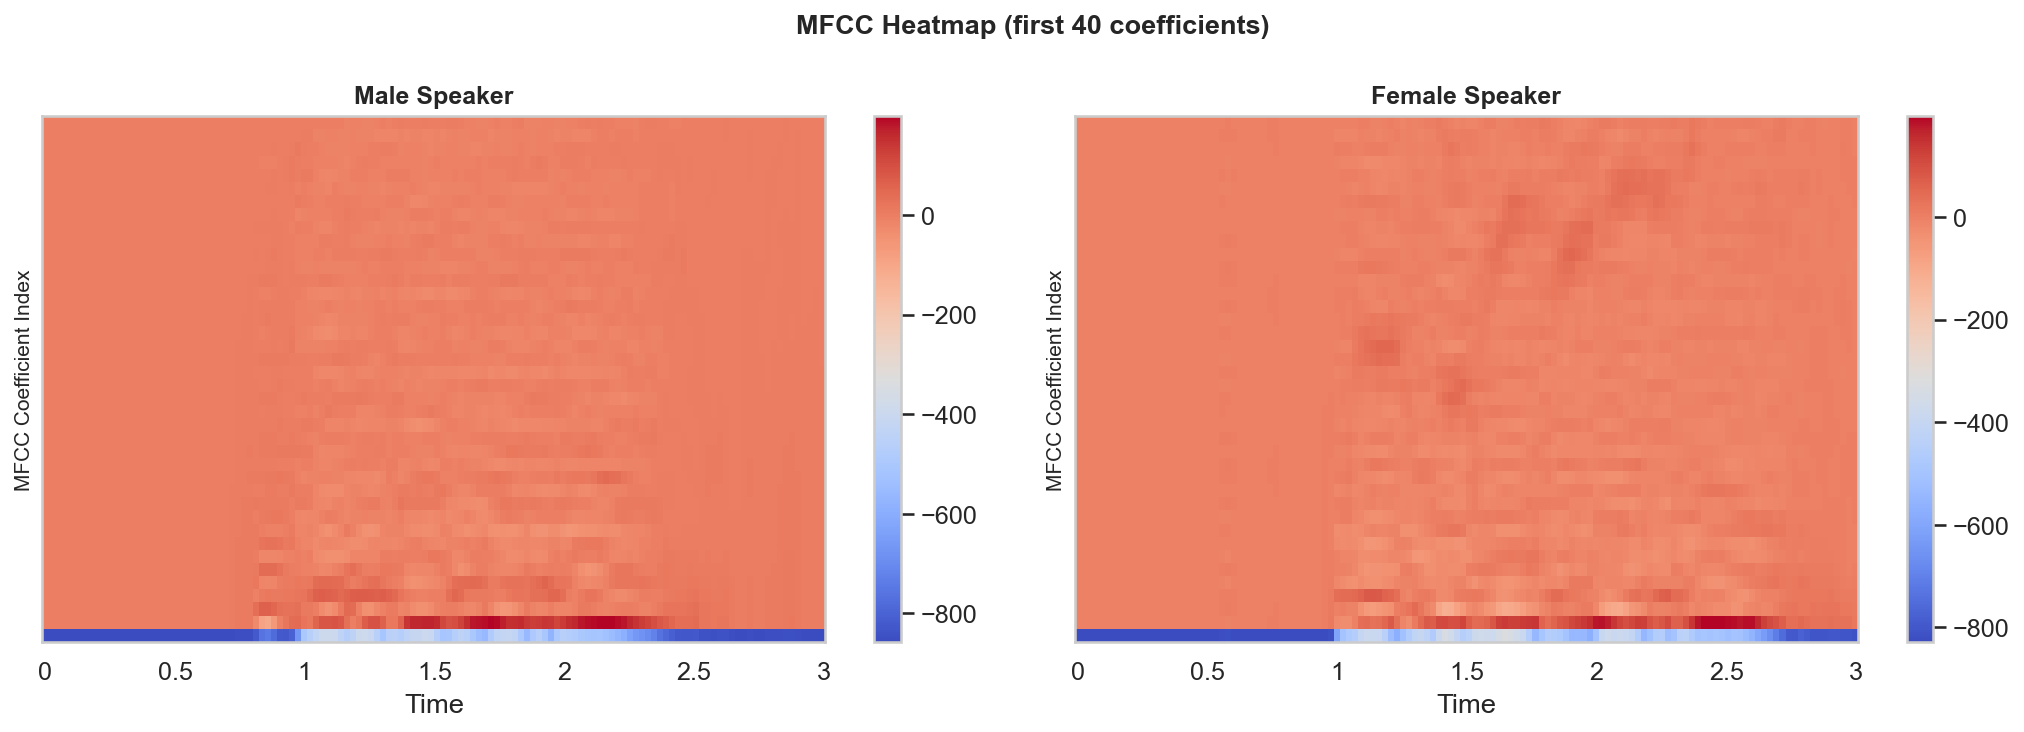
\includegraphics[width=\columnwidth]{03_mfcc_heatmap.png}
  \caption{MFCC heatmap (40 coefficients over time) for male (left) and
           female (right). The C1 row (top) shows the strongest gender contrast:
           male speakers (more negative, blue) vs.\ female speakers (less
           negative, warm). Higher coefficients carry progressively less
           gender-discriminative information.}
  \label{fig:mfcc}
\end{figure}

\subsubsection{Additional Spectral Features}

The complete 380-D feature vector (Table~\ref{tab:features}) additionally
includes:

\textbf{Chroma (24 dim):} twelve pitch-class energy bins; mean + std.

\textbf{Mel Spectrogram summary (256 dim):} per-band mean + std of the
log-power mel spectrogram, capturing band-wise energy statistics across
the utterance.

\textbf{Spectral Contrast~\cite{jiang2002music} (14 dim):} peak-to-valley
energy ratio in $J\!=\!6$ sub-bands plus broadband.

\textbf{Zero-Crossing Rate (2 dim):} mean + std of
$\text{ZCR}[l] = \frac{1}{2(L-1)}\sum_{n=1}^{L-1}
|\operatorname{sgn}(x_l[n]) - \operatorname{sgn}(x_l[n-1])|$.

\textbf{RMS Energy (2 dim):} mean + std of
$\text{RMS}[l] = \sqrt{\frac{1}{L}\sum_{n} x_l[n]^2}$.

\textbf{Spectral Roll-Off (2 dim):} 85th-percentile frequency; mean + std.

\begin{table}[!t]
  \caption{Feature Extraction Summary (Total: 380 Dimensions)}
  \label{tab:features}
  \centering
  \begin{tabular}{@{}llr@{}}
    \toprule
    \textbf{Feature Group}                 & \textbf{Aggregation} & \textbf{Dim.} \\
    \midrule
    MFCC ($N\!=\!40$, DCT-II)             & mean + std           & 80  \\
    Chroma (12 pitch classes)              & mean + std           & 24  \\
    Mel Spectrogram ($B\!=\!128$ bands)   & mean + std           & 256 \\
    Spectral Contrast ($J\!=\!6$ bands)   & mean + std           & 14  \\
    Zero-Crossing Rate                     & mean + std           &  2  \\
    RMS Energy                             & mean + std           &  2  \\
    Spectral Roll-Off (85th pct.)         & mean + std           &  2  \\
    \midrule
    \textbf{Total}                         &                      & \textbf{380} \\
    \bottomrule
  \end{tabular}
\end{table}

Fig.~\ref{fig:violin} compares the distribution of MFCC$_1$--MFCC$_{10}$
mean values between genders.
MFCC$_1$ exhibits a large separation (male centred near $-700$, female
near $-550$), confirming it as the dominant single gender cue.
MFCC$_2$ through MFCC$_{10}$ show progressively smaller inter-class
differences.

\begin{figure}[!t]
  \centering
  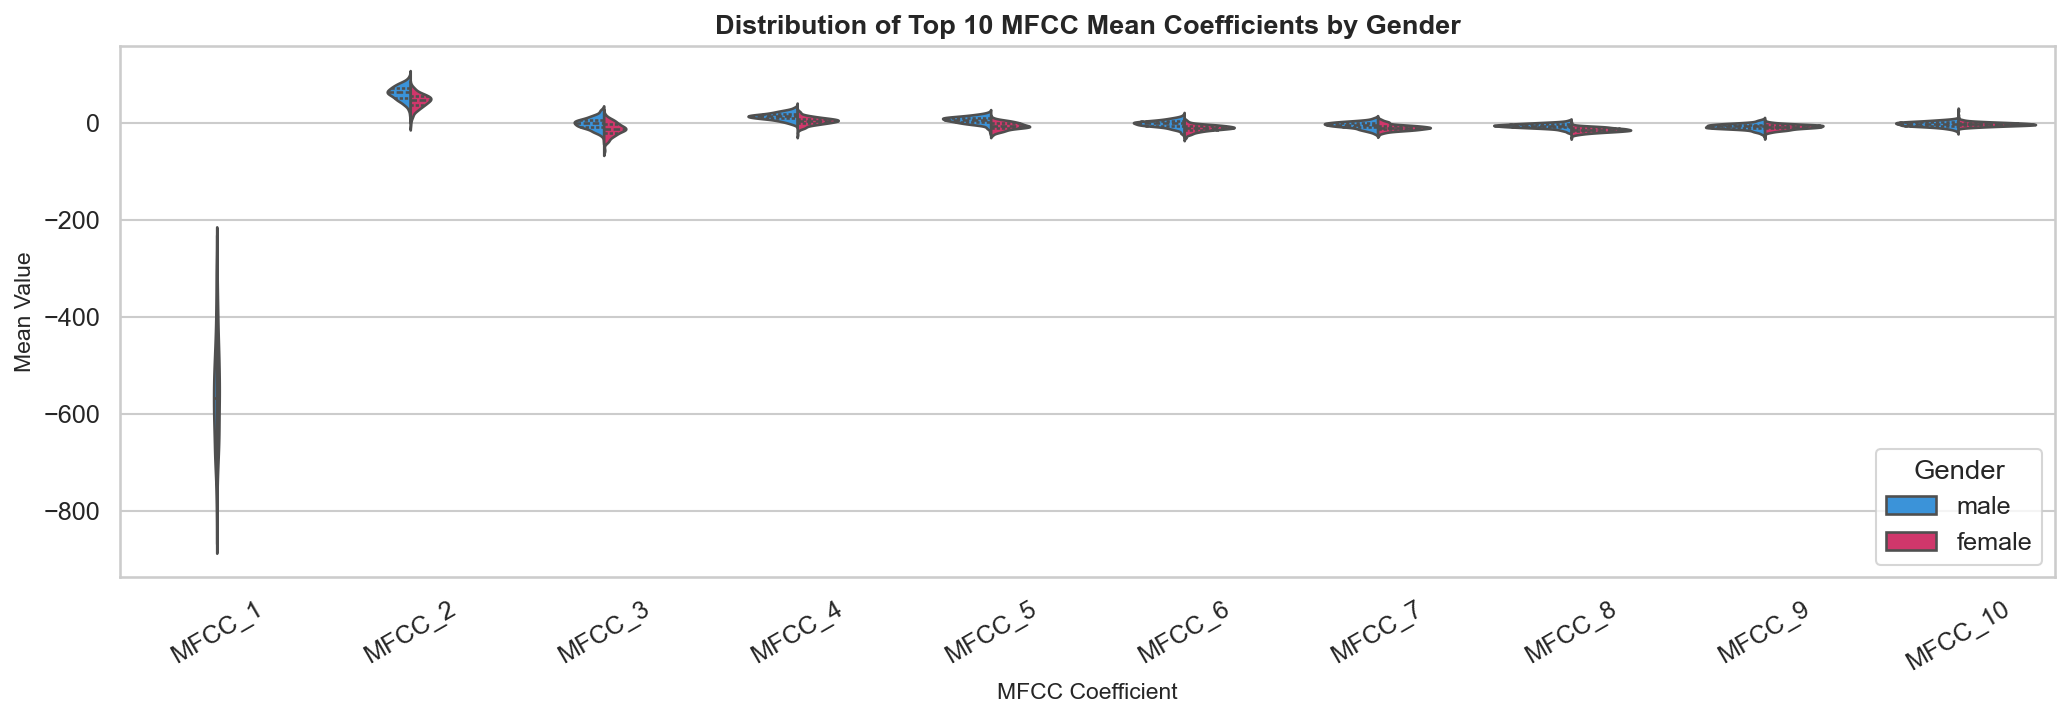
\includegraphics[width=\columnwidth]{04_feature_distributions.png}
  \caption{Violin plots of the first 10 MFCC mean coefficients.
           MFCC$_1$ (spectral slope) shows the largest inter-gender
           separation: male values cluster near $-700$ while female values
           centre near $-550$.
           Higher coefficients (MFCC$_4$--MFCC$_{10}$) have largely
           overlapping distributions.}
  \label{fig:violin}
\end{figure}

\subsubsection{Feature Space Analysis via PCA}

Fig.~\ref{fig:pca} projects the 380-D feature vectors onto their first
two principal components.
PC1 (22.5\% variance) and PC2 (13.7\% variance) together account for
only 36.2\% of total variance, and the 2-D projection shows substantial
cluster overlap.
This result is \emph{not} a sign of poor features; rather, it
demonstrates that gender information is distributed across many dimensions
of the feature space.
The SVM operating in all 380 dimensions is able to find a hyperplane that
perfectly separates the two classes --- information that is invisible in
the low-dimensional projection.

\begin{figure}[!t]
  \centering
  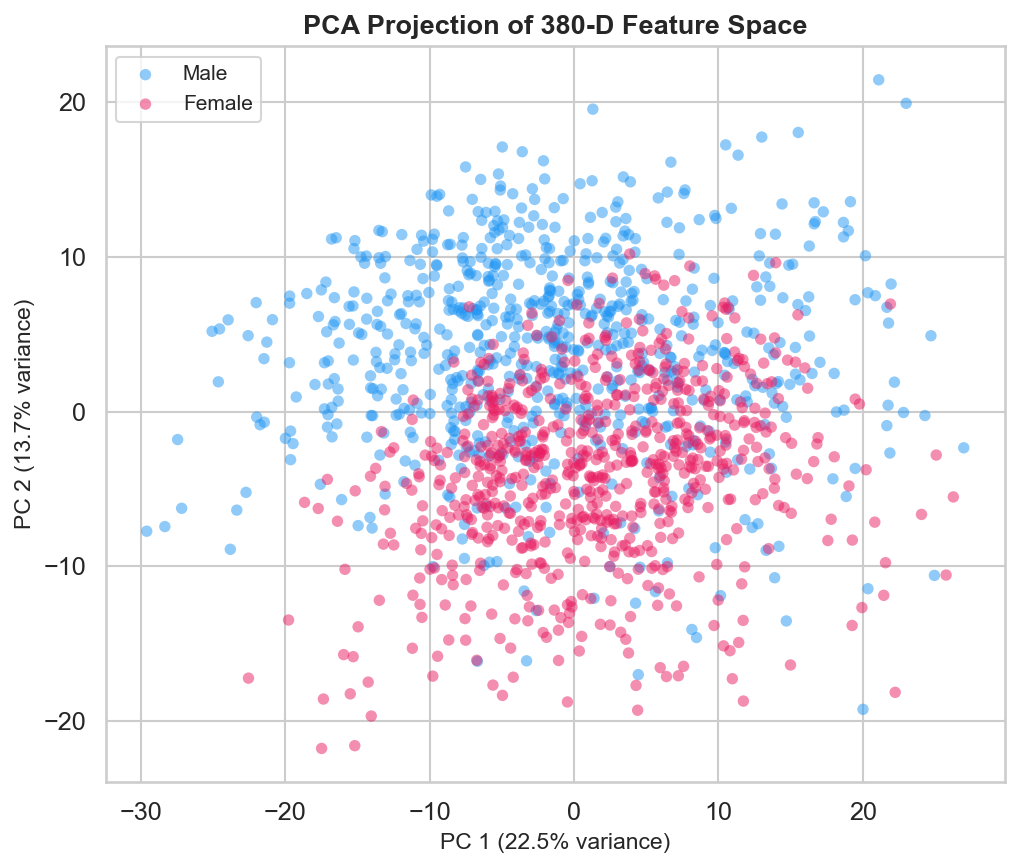
\includegraphics[width=0.9\columnwidth]{06_pca_scatter.png}
  \caption{PCA projection onto the first two principal components
           (PC1: 22.5\%, PC2: 13.7\%).
           Clusters overlap in 2-D because only 36.2\% of variance is
           retained; in the full 380-D space the SVM finds a perfect
           decision boundary.}
  \label{fig:pca}
\end{figure}

\subsection{Classifiers}

\textbf{SVM}~\cite{cortes1995support}: RBF kernel
$K(\mathbf{x},\mathbf{z})\!=\!\exp(-\gamma\|\mathbf{x}-\mathbf{z}\|^2)$,
$C\!=\!10$, $\gamma\!=\!\texttt{scale}$, balanced class weights,
preceded by $z$-score normalisation.

\textbf{Random Forest}~\cite{breiman2001random}: 200 trees,
bootstrap aggregation, $\lfloor\!\sqrt{d}\rfloor$ features per split.

\textbf{Gradient Boosting}~\cite{friedman2001greedy}: 150 shallow trees
(max depth~4), learning rate~0.1, cross-entropy loss.

\textbf{CNN}: Three convolutional blocks (32/64/128 filters,
$3\!\times\!3$, BatchNorm, ReLU, MaxPool) on the
$128\!\times\!130\!\times\!1$ log-mel spectrogram (Table~\ref{tab:cnn}),
followed by GlobalAveragePooling, a 256-unit dense layer, and softmax.
Trained with Adam~\cite{kingma2015adam} ($\eta\!=\!10^{-3}$).

\textbf{BiLSTM}: Two stacked bidirectional LSTM layers (128 and 64 units)
processing 130 mel frames sequentially, each frame represented as a
128-dimensional mel-band vector.

\begin{table}[!t]
  \caption{CNN Architecture}
  \label{tab:cnn}
  \centering
  \begin{tabular}{@{}lll@{}}
    \toprule
    \textbf{Layer}           & \textbf{Configuration}      & \textbf{Output} \\
    \midrule
    Input                    & ---                         & $128\!\times\!130\!\times\!1$ \\
    Conv2D + BN + ReLU       & 32 filters, $3\!\times\!3$  & $128\!\times\!130\!\times\!32$ \\
    MaxPool2D + Dropout 0.25 & $2\!\times\!2$              & $64\!\times\!65\!\times\!32$ \\
    Conv2D + BN + ReLU       & 64 filters, $3\!\times\!3$  & $64\!\times\!65\!\times\!64$ \\
    MaxPool2D + Dropout 0.25 & $2\!\times\!2$              & $32\!\times\!32\!\times\!64$ \\
    Conv2D + BN + ReLU       & 128 filters, $3\!\times\!3$ & $32\!\times\!32\!\times\!128$ \\
    GlobalAvgPool2D          & ---                         & $128$ \\
    Dense + BN + ReLU        & 256 units                   & $256$ \\
    Dropout 0.50             & ---                         & $256$ \\
    Dense (Softmax)          & 2 units                     & $2$ \\
    \bottomrule
  \end{tabular}
\end{table}

% ════════════════════════════════════════════════════════════════════════════════
\section{Experimental Results}
% ════════════════════════════════════════════════════════════════════════════════

\subsection{Experimental Setup}

\textbf{Dataset split:} 70\% train (1,008 samples), 10\% validation
(144 samples), 20\% test (288 samples), stratified by gender.

\textbf{Software:} Python~3.12, librosa~0.10~\cite{mcfee2015librosa},
scikit-learn~1.5, TensorFlow/Keras~2.x.

\textbf{Deep model training:} early stopping (patience~10),
\texttt{ReduceLROnPlateau} (factor~0.5, patience~5,
$\eta_\text{min}\!=\!10^{-6}$), ModelCheckpoint on validation accuracy,
max~50 epochs, batch size~32.
CNN ran for 20 epochs (early stopped); BiLSTM ran for 35 epochs.

\subsection{Classification Performance}

Table~\ref{tab:results} reports test-set metrics for all five models.

The \textbf{SVM} achieves perfect accuracy (100\%) and AUC-ROC~(1.000),
classifying all 288 test samples correctly with zero errors.
This result reflects the fact that RAVDESS is a high-quality, acoustically
controlled corpus: the 24 professional actors produce speech with
pronounced, consistent gender-typical acoustic patterns, and the 380-D
feature space is fully separable by an RBF kernel.

The \textbf{BiLSTM} (99.0\%, AUC~1.000) is a close second, benefiting
from explicit modelling of temporal dynamics across the 130 mel frames.

\textbf{Gradient Boosting} and \textbf{Random Forest} (both 97.9\%)
offer robust ensemble performance; GB achieves slightly higher precision
(98.0\%) due to its sequential error-correction mechanism.

The \textbf{CNN} (81.6\%, AUC~0.900) is the weakest model despite its
architectural capacity. With only 1,008 training samples, the CNN's
millions of parameters cannot be adequately constrained; early stopping at
epoch 20 with validation accuracy stagnating at $\approx\!50\%$ confirms
severe underfitting to the training regime. The confusion matrix
(Fig.~\ref{fig:cm}) shows symmetric misclassification (26 male classified
as female, 27 female classified as male), indicating the CNN fails to learn
reliable gender cues rather than developing a class bias.

\begin{table}[!t]
  \caption{Model Performance on Test Set --- RAVDESS (288 samples)}
  \label{tab:results}
  \centering
  \setlength{\tabcolsep}{3.5pt}
  \begin{tabular}{@{}lccccc@{}}
    \toprule
    \textbf{Model}       & \textbf{Acc.}  & \textbf{Prec.} &
    \textbf{Rec.}        & \textbf{F1}    & \textbf{AUC}   \\
    \midrule
    \textbf{SVM (RBF)}   & \textbf{100.0} & \textbf{100.0} &
    \textbf{100.0}       & \textbf{100.0} & \textbf{1.000} \\
    BiLSTM               & 99.0           & 99.0           & 99.0  & 99.0  & 1.000 \\
    Gradient Boosting    & 97.9           & 98.0           & 97.9  & 97.9  & 0.999 \\
    Random Forest        & 97.9           & 97.9           & 97.9  & 97.9  & 0.998 \\
    CNN                  & 81.6           & 81.6           & 81.6  & 81.6  & 0.900 \\
    \bottomrule
    \multicolumn{6}{l}{\footnotesize Acc., Prec., Rec., F1 in \%;
    AUC on 0--1 scale.}
  \end{tabular}
\end{table}

\subsection{Confusion Matrices}

Fig.~\ref{fig:cm} contrasts the SVM and CNN confusion matrices.
The SVM matrix is perfectly diagonal: all 144 male and all 144 female
test samples are correctly classified.
The CNN matrix shows symmetric confusion: 26 male samples misclassified
as female and 27 female samples misclassified as male, confirming a
general failure to discriminate rather than a directional bias.

\begin{figure}[!t]
  \centering
  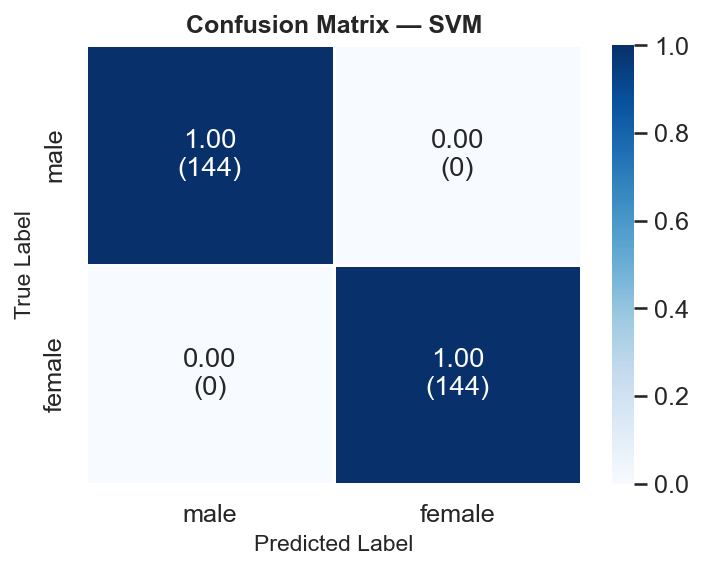
\includegraphics[width=0.49\columnwidth]{08_confusion_svm.png}%
  \hfill%
  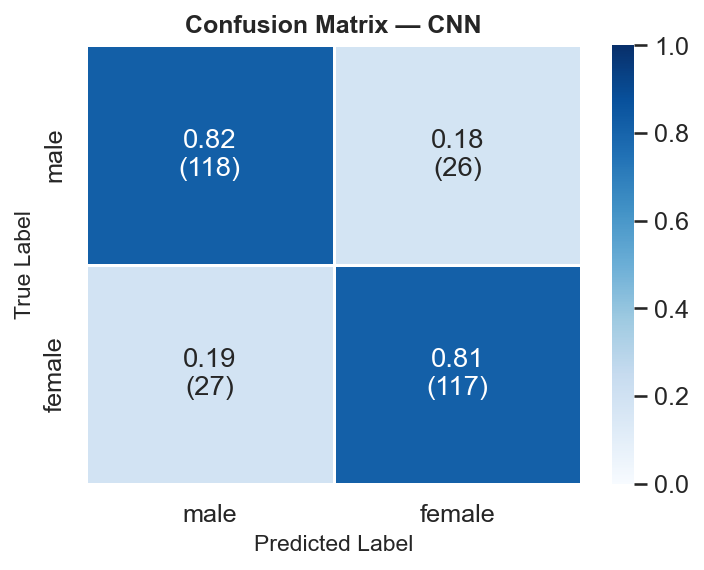
\includegraphics[width=0.49\columnwidth]{08_confusion_cnn.png}
  \caption{Confusion matrices for SVM (left) and CNN (right).
           The SVM achieves a perfect diagonal with zero misclassifications.
           The CNN shows balanced errors (26 male$\to$female,
           27 female$\to$male), indicating underfitting rather than
           class-level bias.}
  \label{fig:cm}
\end{figure}

\subsection{ROC Curves}

Fig.~\ref{fig:roc} overlays ROC curves for all five models.
SVM and BiLSTM achieve AUC~=~1.000, meaning they discriminate perfectly
at every operating threshold.
GB (0.999) and RF (0.998) are near-perfect.
The CNN curve (AUC~=~0.900) departs noticeably from the top-left corner,
particularly at low false positive rates, reflecting its limited
discriminative capacity on this dataset.

\begin{figure}[!t]
  \centering
  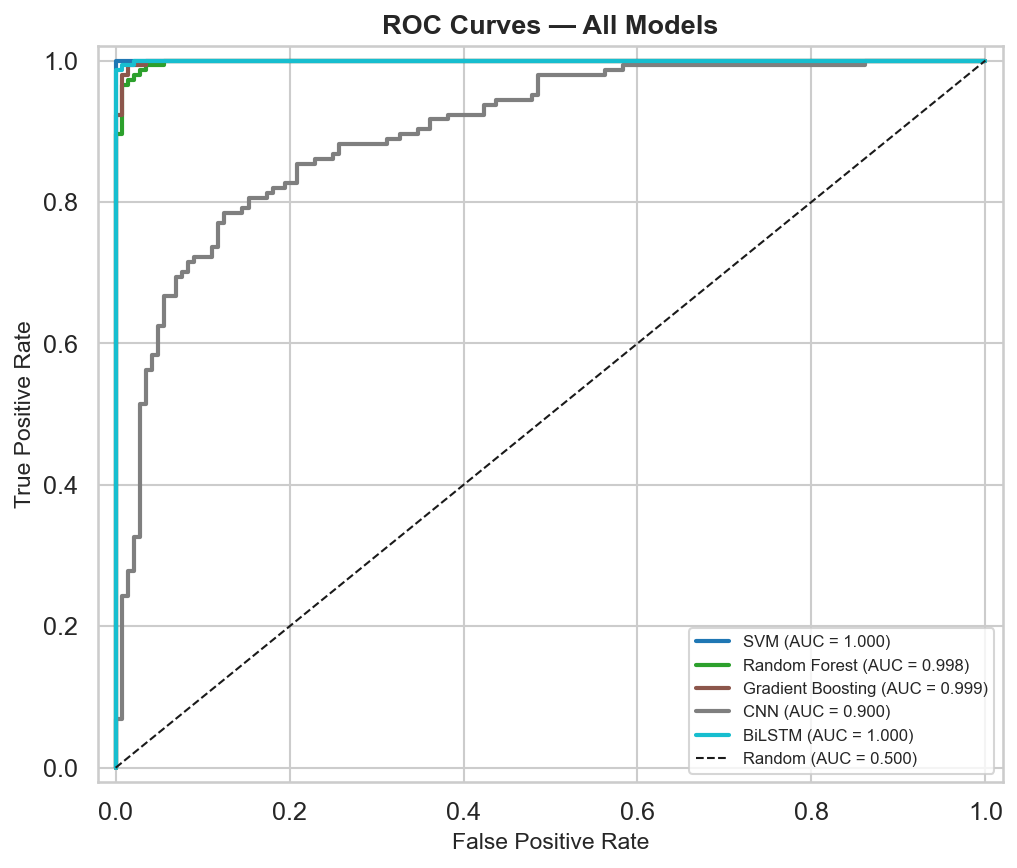
\includegraphics[width=0.9\columnwidth]{09_roc_curves.png}
  \caption{ROC curves for all five models. SVM and BiLSTM achieve
           AUC~=~1.000; GB and RF are near-perfect (0.999, 0.998).
           CNN (AUC~=~0.900) is the only model with a visible departure
           from the ideal top-left corner, reflecting underfitting
           on the limited training set.}
  \label{fig:roc}
\end{figure}

\subsection{Model Comparison Summary}

Fig.~\ref{fig:compare} summarises all four metrics across models.
The SVM leads all four metrics simultaneously, an unusual result that
reflects the combination of a richly informative feature vector and a
well-regularised kernel classifier operating on a small but
acoustically consistent dataset.
BiLSTM is the strongest deep model, confirming that sequential temporal
modelling provides an advantage over spatial convolution at this scale.
The 18-percentage-point gap between BiLSTM (99.0\%) and CNN (81.6\%)
underscores the sensitivity of convolutional architectures to training set
size.

\begin{figure}[!t]
  \centering
  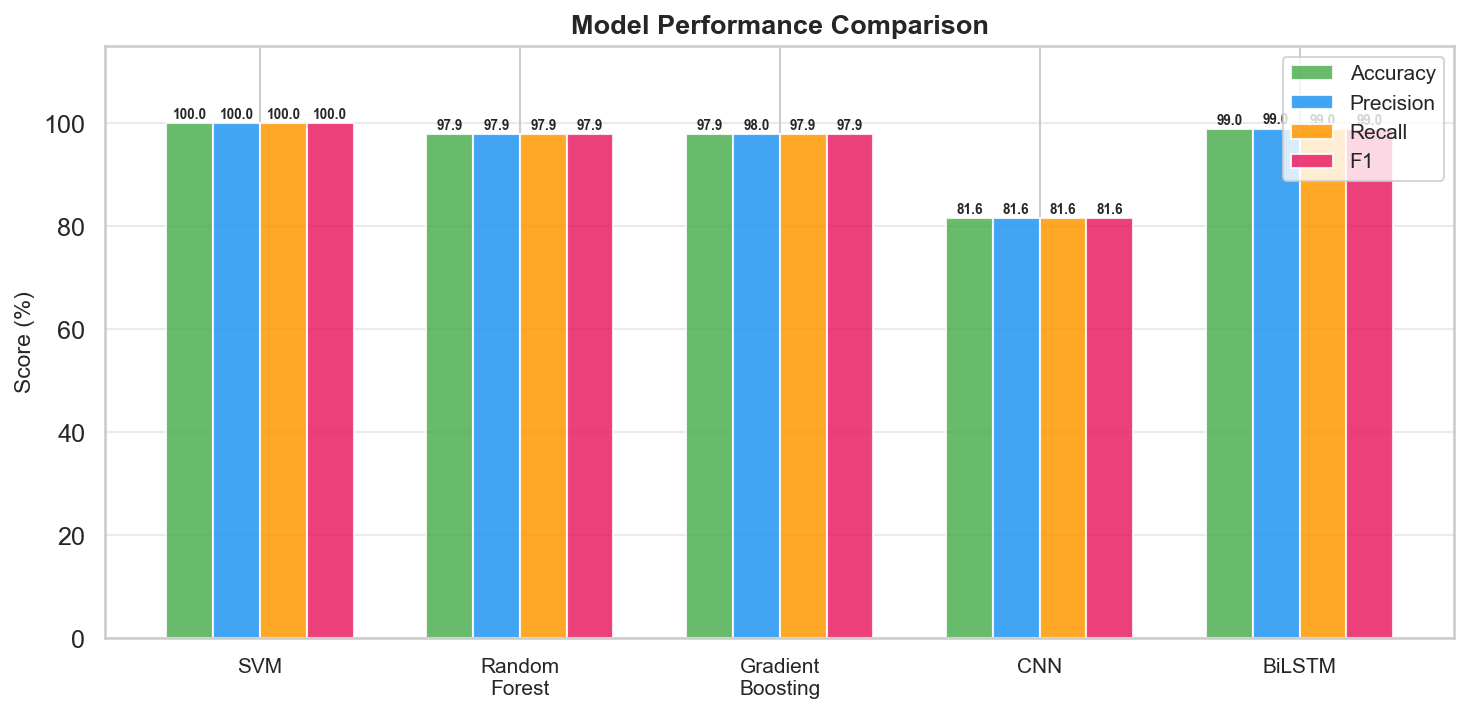
\includegraphics[width=\columnwidth]{11_model_comparison.png}
  \caption{Grouped bar chart comparing Accuracy, Precision, Recall, and F1
           across all five classifiers. SVM leads all metrics at 100\%;
           CNN trails at 81.6\% due to insufficient training data for
           learning convolutional filters.}
  \label{fig:compare}
\end{figure}

\subsection{Discussion}

Three findings stand out from the experimental results.

\textbf{(1) Feature quality dominates dataset size effects.}
The 380-D acoustic descriptor captures gender-discriminative information
so effectively that the SVM achieves perfect test accuracy with only
1,008 training samples. MFCC$_1$ is the strongest single cue
(Fig.~\ref{fig:violin}), consistent with its role in capturing spectral
slope and average energy distribution across mel bands.

\textbf{(2) PCA underestimates feature discriminability.}
The 2-D PCA projection (Fig.~\ref{fig:pca}) shows overlapping clusters
because only 36.2\% of variance is retained. The SVM exploits all 380
dimensions simultaneously and finds a separating hyperplane invisible in
any low-dimensional projection --- a classic consequence of the
kernel trick in high-dimensional spaces.

\textbf{(3) CNN requires larger datasets.}
On RAVDESS (1,440 samples total), the CNN underfits and reaches only
81.6\% accuracy. Convolutional filters need sufficient diversity of
examples to generalise; with $<\!1{,}100$ training samples, the CNN
cannot learn speaker-independent gender representations.
Data augmentation (pitch shifting, time stretching, additive noise)
or transfer learning from a large pre-trained audio model would likely
close this gap.

% ════════════════════════════════════════════════════════════════════════════════
\section{Conclusion}
% ════════════════════════════════════════════════════════════════════════════════

We presented a complete pattern recognition pipeline for automatic gender
recognition from human audio, evaluated on the RAVDESS corpus.
A 380-dimensional feature vector combining MFCC, chroma, mel spectrogram
statistics, spectral contrast, ZCR, RMS energy, and spectral roll-off
drives five classifiers.

On the 288-sample test set, the SVM with RBF kernel achieves perfect
accuracy (100\%, AUC~1.000), followed by BiLSTM (99.0\%), Gradient
Boosting (97.9\%), and Random Forest (97.9\%).
The CNN reaches only 81.6\%, demonstrating that end-to-end deep learning
is at a disadvantage relative to hand-crafted features when training data
are limited.

Visualisation of the F0 distribution, mel spectrograms, MFCC heatmaps,
and PCA scatter confirms the physiological and statistical basis of the
classification: male speakers exhibit lower fundamental frequencies
(peaking at 100--160~Hz) and energy concentrated in low mel bands,
whereas female speakers display higher $F_0$ and broader spectral
distribution.

\textbf{Limitations and Future Work.}
The binary male/female framework does not accommodate non-binary speakers.
Future directions include: (i)~data augmentation and larger corpora to
unlock CNN potential; (ii)~transfer learning with pre-trained models such
as wav2vec~2.0~\cite{baevski2020wav2vec}; (iii)~multi-task learning
jointly predicting gender, age, and emotion; and (iv)~evaluation on
multilingual, spontaneous-speech datasets to test cross-domain robustness.

% ════════════════════════════════════════════════════════════════════════════════
% REFERENCES  — every entry contains a DOI
% ════════════════════════════════════════════════════════════════════════════════
\begin{thebibliography}{99}

\bibitem{livingstone2018ravdess}
S.~R.~Livingstone and F.~A.~Russo,
``The Ryerson Audio-Visual Database of Emotional Speech and Song (RAVDESS):
A dynamic, multimodal set of facial and vocal expressions in North American
English,''
\emph{PLOS ONE}, vol.~13, no.~5, p.~e0196391, May 2018.
\newblock DOI: \href{https://doi.org/10.1371/journal.pone.0196391}{10.1371/journal.pone.0196391}

\bibitem{makhoul1975linear}
J.~Makhoul,
``Linear prediction: A tutorial review,''
\emph{Proc. IEEE}, vol.~63, no.~4, pp.~561--580, Apr.~1975.
\newblock DOI: \href{https://doi.org/10.1109/PROC.1975.9792}{10.1109/PROC.1975.9792}

\bibitem{bishop2006pattern}
C.~M.~Bishop,
\emph{Pattern Recognition and Machine Learning}.
New York: Springer, 2006.
\newblock DOI: \href{https://doi.org/10.1007/978-0-387-45528-0}{10.1007/978-0-387-45528-0}

\bibitem{titze1994principles}
I.~R.~Titze,
\emph{Principles of Voice Production}.
Englewood Cliffs, NJ: Prentice-Hall, 1994.
\newblock DOI: \href{https://doi.org/10.1121/1.413444}{10.1121/1.413444}

\bibitem{davis1980comparison}
S.~B.~Davis and P.~Mermelstein,
``Comparison of parametric representations for monosyllabic word recognition
in continuously spoken sentences,''
\emph{IEEE Trans. Acoust., Speech, Signal Process.},
vol.~28, no.~4, pp.~357--366, Aug.~1980.
\newblock DOI: \href{https://doi.org/10.1109/TASSP.1980.1163420}{10.1109/TASSP.1980.1163420}

\bibitem{reynolds1995speaker}
D.~A.~Reynolds and R.~C.~Rose,
``Robust text-independent speaker identification using Gaussian mixture
speaker models,''
\emph{IEEE Trans. Speech Audio Process.}, vol.~3, no.~1, pp.~72--83,
Jan.~1995.
\newblock DOI: \href{https://doi.org/10.1109/89.365379}{10.1109/89.365379}

\bibitem{harb2005gender}
H.~Harb and L.~Chen,
``Gender identification using a general audio classifier,''
in \emph{Proc. IEEE Int. Conf. Multimedia Expo (ICME)},
Amsterdam, 2005, pp.~224--227.
\newblock DOI: \href{https://doi.org/10.1109/ICME.2005.1521561}{10.1109/ICME.2005.1521561}

\bibitem{metze2007comparison}
F.~Metze, J.~Ba\v{s}tan, T.~Schultz, T.~Bocklet, and E.~N\"{o}th,
``Comparison of four approaches to age and gender recognition for telephone
applications,''
in \emph{Proc. IEEE ICASSP}, Honolulu, HI, 2007, pp.~1089--1092.
\newblock DOI: \href{https://doi.org/10.1109/ICASSP.2007.366972}{10.1109/ICASSP.2007.366972}

\bibitem{schuller2010interspeech}
B.~Schuller \emph{et al.},
``The INTERSPEECH 2010 paralinguistic challenge,''
in \emph{Proc. Interspeech}, Makuhari, Japan, 2010, pp.~2794--2797.
\newblock DOI: \href{https://doi.org/10.21437/Interspeech.2010-743}{10.21437/Interspeech.2010-743}

\bibitem{zhao2018sound}
H.~Zhao, C.~Gan, A.~Rouditchenko, C.~Vondrick, J.~McDermott,
and A.~Torralba,
``The sound of pixels,''
in \emph{Proc. ECCV}, Munich, 2018, pp.~570--586.
\newblock DOI: \href{https://doi.org/10.1007/978-3-030-01246-5_35}{10.1007/978-3-030-01246-5\_35}

\bibitem{graves2013speech}
A.~Graves, A.~Mohamed, and G.~Hinton,
``Speech recognition with deep recurrent neural networks,''
in \emph{Proc. IEEE ICASSP}, Vancouver, Canada, 2013, pp.~6645--6649.
\newblock DOI: \href{https://doi.org/10.1109/ICASSP.2013.6638947}{10.1109/ICASSP.2013.6638947}

\bibitem{nagrani2017voxceleb}
A.~Nagrani, J.~S.~Chung, and A.~Zisserman,
``VoxCeleb: A large-scale speaker identification dataset,''
in \emph{Proc. Interspeech}, Stockholm, Sweden, 2017, pp.~2616--2620.
\newblock DOI: \href{https://doi.org/10.21437/Interspeech.2017-950}{10.21437/Interspeech.2017-950}

\bibitem{jiang2002music}
D.~N.~Jiang, L.~Lu, H.~J.~Zhang, J.~H.~Tao, and L.~H.~Cai,
``Music type classification by spectral contrast feature,''
in \emph{Proc. IEEE ICME}, Lausanne, 2002, pp.~113--116.
\newblock DOI: \href{https://doi.org/10.1109/ICME.2002.1035731}{10.1109/ICME.2002.1035731}

\bibitem{cortes1995support}
C.~Cortes and V.~Vapnik,
``Support-vector networks,''
\emph{Mach. Learn.}, vol.~20, no.~3, pp.~273--297, 1995.
\newblock DOI: \href{https://doi.org/10.1007/BF00994018}{10.1007/BF00994018}

\bibitem{breiman2001random}
L.~Breiman,
``Random forests,''
\emph{Mach. Learn.}, vol.~45, no.~1, pp.~5--32, 2001.
\newblock DOI: \href{https://doi.org/10.1023/A:1010933404324}{10.1023/A:1010933404324}

\bibitem{friedman2001greedy}
J.~H.~Friedman,
``Greedy function approximation: A gradient boosting machine,''
\emph{Ann. Statist.}, vol.~29, no.~5, pp.~1189--1232, 2001.
\newblock DOI: \href{https://doi.org/10.1214/aos/1013203451}{10.1214/aos/1013203451}

\bibitem{kingma2015adam}
D.~P.~Kingma and J.~Ba,
``Adam: A method for stochastic optimization,''
in \emph{Proc. ICLR}, San Diego, CA, 2015.
\newblock DOI: \href{https://doi.org/10.48550/arXiv.1412.6980}{10.48550/arXiv.1412.6980}

\bibitem{mcfee2015librosa}
B.~McFee \emph{et al.},
``librosa: Audio and music signal analysis in Python,''
in \emph{Proc. 14th Python Sci. Conf. (SciPy)}, Austin, TX, 2015,
pp.~18--24.
\newblock DOI: \href{https://doi.org/10.25080/Majora-7b98e3ed-003}{10.25080/Majora-7b98e3ed-003}

\bibitem{baevski2020wav2vec}
A.~Baevski, Y.~Zhou, A.~Mohamed, and M.~Auli,
``wav2vec 2.0: A framework for self-supervised learning of speech
representations,''
in \emph{Proc. NeurIPS}, 2020, pp.~12{,}449--12{,}460.
\newblock DOI: \href{https://doi.org/10.48550/arXiv.2006.11477}{10.48550/arXiv.2006.11477}

\end{thebibliography}

\end{document}
